\documentclass[tikz,border=6pt]{standalone}
\usetikzlibrary{arrows.meta}

\definecolor{KetteringBlue}{HTML}{1E4B99}

\begin{document}
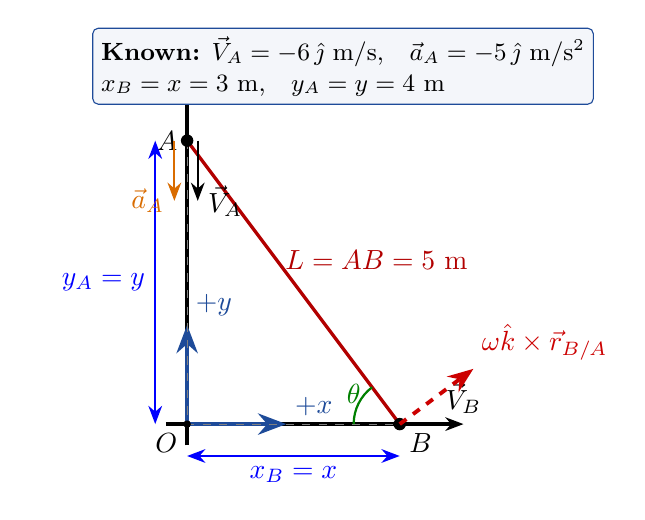
\begin{tikzpicture}[scale=0.9, >=Stealth]
    % White background so Markdown previews do not hide black labels.
    \fill[white] (-2.25,-0.85) rectangle (5.15,5.45);

    % Coordinates
    \coordinate (O) at (0,0);
    \coordinate (A) at (0,4);
    \coordinate (B) at (3,0);

    % Wall and floor
    \draw[very thick] (0,-0.3) -- (0,4.7);
    \draw[very thick] (-0.3,0) -- (3.8,0);

    % Coordinate axes from O (drawn on top of wall/floor in distinct color)
    \draw[->, line width=1.6pt, KetteringBlue] (O) -- (1.4,0)
        node[KetteringBlue, above right=-1pt] {$+x$};
    \draw[->, line width=1.6pt, KetteringBlue] (O) -- (0,1.4)
        node[KetteringBlue, above right=-1pt] {$+y$};

    % Constraint triangle
    \draw[dashed, gray] (A) -- (O) -- (B);
    \draw[very thick, red!70!black] (A) -- (B);

    % Points
    \fill (A) circle (2.5pt) node[left] {$A$};
    \fill (B) circle (2.5pt) node[below right] {$B$};
    \fill (O) circle (1.5pt) node[below left] {$O$};

    % Known values
    \node[
        draw=KetteringBlue,
        rounded corners=2pt,
        fill=KetteringBlue!5,
        align=left,
        inner sep=3pt,
        font=\small
    ] at (2.2,5.05) {%
        \textbf{Known:}
        $\vec V_A=-6\,\hat{\jmath}\ \mathrm{m/s}$,\quad
        $\vec a_A=-5\,\hat{\jmath}\ \mathrm{m/s^2}$\\
        $x_B=x=3\ \mathrm{m}$,\quad
        $y_A=y=4\ \mathrm{m}$%
    };

    % Dimension arrows
    \draw[<->, blue, thick] (0,-0.45) -- node[below] {$x_B=x$} (3,-0.45);
    \draw[<->, blue, thick] (-0.45,0) -- node[left] {$y_A=y$} (-0.45,4);

    % Rod length label
    \node[red!70!black, above right] at (1.25,2.05) {$L=AB=5\ \mathrm{m}$};

    % Angle
    \draw[green!50!black, thick] (2.35,0) arc[start angle=180, end angle=126.87, radius=0.65];
    \node[green!50!black] at (2.35,0.42) {$\theta$};

    % Velocity and acceleration directions
    \draw[->, thick] (0.15,4) -- ++(0,-0.85)
        node[right] {$\vec V_A$};
    \draw[->, thick, orange!85!black] (-0.18,4) -- ++(0,-0.85)
        node[left] {$\vec a_A$};
    \draw[->, thick] (B) -- ++(0.9,0) node[above] {$\vec V_B$};

    % Relative velocity contribution, normal to AB.
    \draw[->, dashed, line width=1.4pt, red!80!black] (B) -- ++(1.04,0.78)
        node[above right=-1pt] {$\omega\hat{k}\times\vec r_{B/A}$};
\end{tikzpicture}
\end{document}
